\documentclass{standalone}
\usepackage[utf8]{inputenc}
\usepackage{amsmath}
\usepackage{amsfonts}
\usepackage{amssymb}
\usepackage{tikz}
\usetikzlibrary{calc}

% GanttHeader setups some parameters for the rest of the diagram
% #1 Width of the diagram
% #2 Width of the space reserved for task numbers
% #3 Width of the space reserved for task names
% #4 Number of months in the diagram
% In addition to these parameters, the layout of the diagram is influenced
% by keys defined below, such as y, which changes the vertical scale
\def\GanttHeader#1#2#3#4{%
 \pgfmathparse{(#1-#2-#3)/(#4)}
 \tikzset{y=7mm, task number/.style={left, font=\bfseries},
     task description/.style={text width=#3,  right, draw=none,
           font=\sffamily, xshift=#2,
           minimum height=2em},
     gantt bar/.style={draw=black, fill=blue!30},
     help lines/.style={draw=black!30, dashed},
     x=\pgfmathresult pt
     }
  \def\totalmonths{#4}
  \node (Header) [task description] at (0,0) {\textbf{\large }};
  \begin{scope}[shift=($(Header.south east)$)]
    \foreach \x in {1,...,#4}
      \node[above,rotate=90] at (\x,1) {\tiny\x};
 \end{scope}
}

% This macro adds a task to the diagram
% #1 Number of the task
% #2 Task's name
% #3 Starting date of the task (month's number, can be non-integer)
% #4 Task's duration in months (can be non-integer)
\def\Task#1#2#3#4{%
%\node[task number] at ($(Header.west) + (0, -#1)$) {#1};
\node[task description] at (0,-#1) {#2};
\begin{scope}[shift=($(Header.south east)$)]
  \draw (0,-#1) rectangle +(\totalmonths, 1);
  \foreach \x in {1,...,\totalmonths}
    \draw[help lines] (\x,-#1) -- +(0,1);
  \filldraw[gantt bar] ($(#3, -#1+0.2)$) rectangle +(#4,0.6);
\end{scope}
}

\begin{document}

\begin{tabular}{lr}
Scheduler: & RR-2 scheduler
\\
Input: & input/testdata2.txt
\\
Total Process Count: & 11
\\
Total Waiting Time: & 752
\\
Average Waiting Time: & 68.36364
\\
Total Turnaround Time: & 884
\\
Average Turnaround Time: & 80.36364
\\
Total Context Switch Count: & 65
\\
\end{tabular}
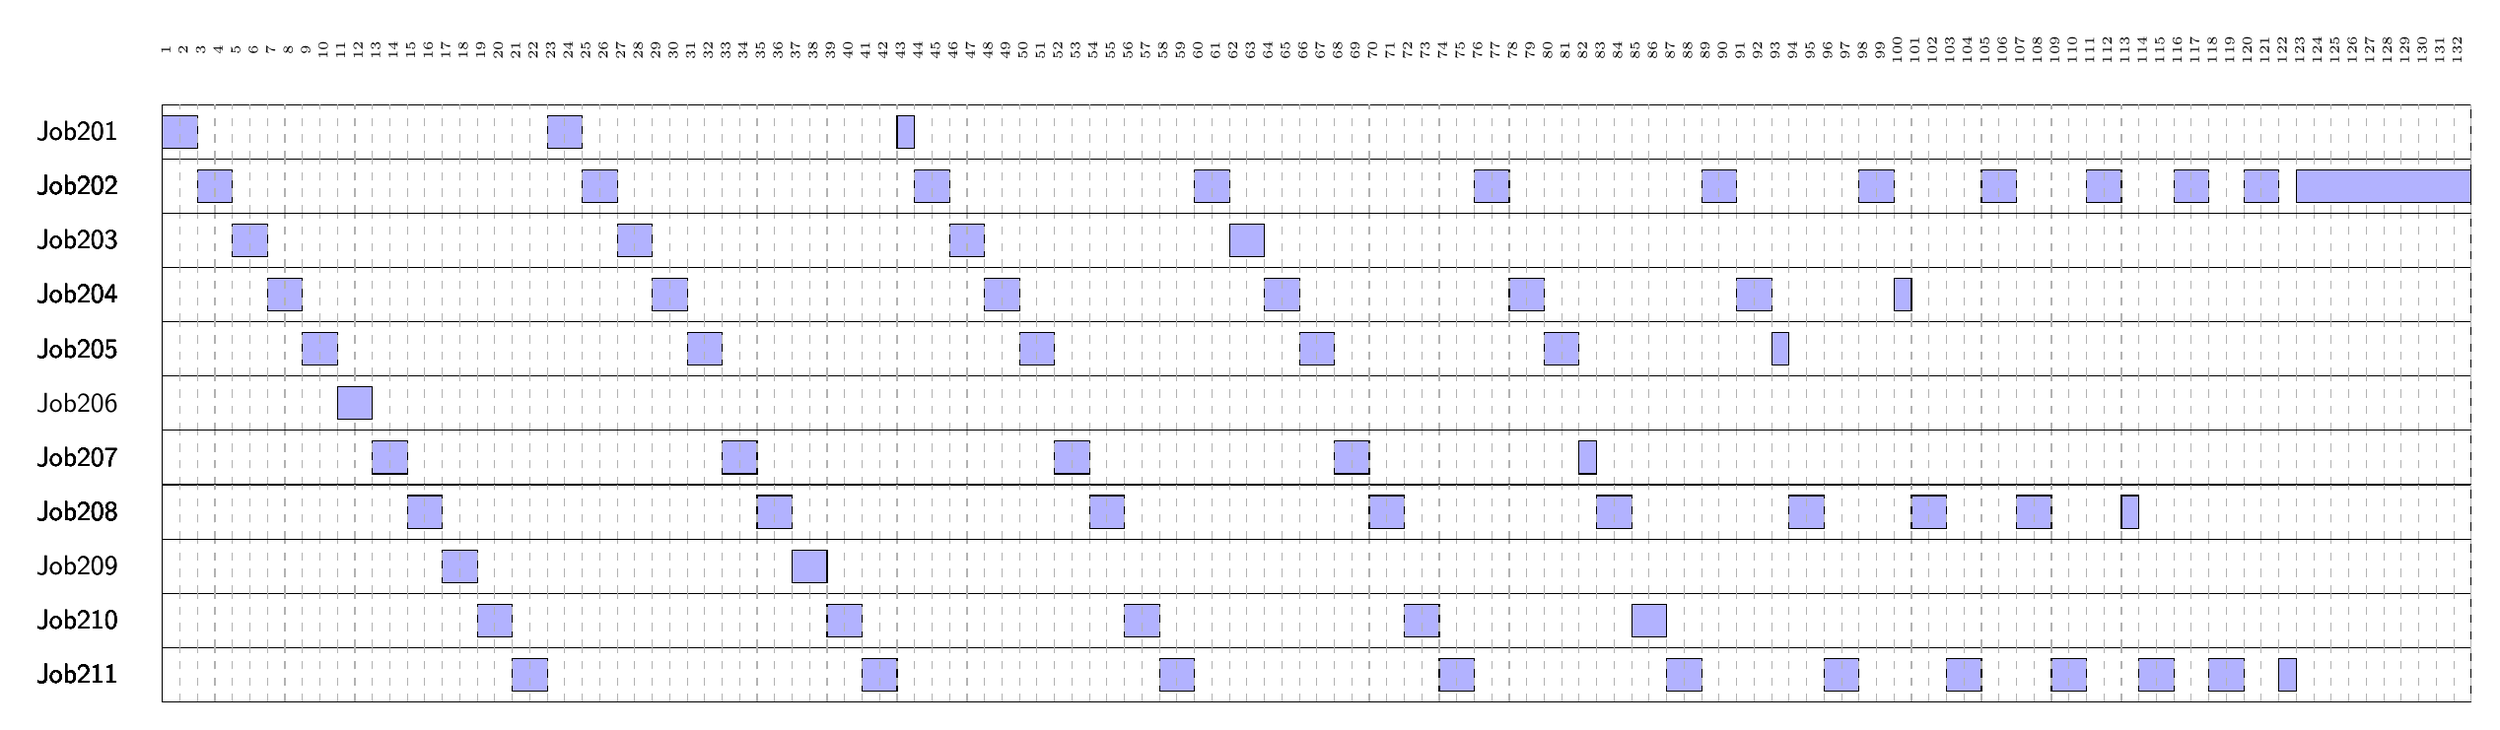
\begin{tikzpicture}
\GanttHeader{32cm}{5ex}{1.5cm}{132}
\Task{1}{Job201}{0}{2}
\Task{2}{Job202}{2}{2}
\Task{3}{Job203}{4}{2}
\Task{4}{Job204}{6}{2}
\Task{5}{Job205}{8}{2}
\Task{6}{Job206}{10}{2}
\Task{7}{Job207}{12}{2}
\Task{8}{Job208}{14}{2}
\Task{9}{Job209}{16}{2}
\Task{10}{Job210}{18}{2}
\Task{11}{Job211}{20}{2}
\Task{1}{Job201}{22}{2}
\Task{2}{Job202}{24}{2}
\Task{3}{Job203}{26}{2}
\Task{4}{Job204}{28}{2}
\Task{5}{Job205}{30}{2}
\Task{7}{Job207}{32}{2}
\Task{8}{Job208}{34}{2}
\Task{9}{Job209}{36}{2}
\Task{10}{Job210}{38}{2}
\Task{11}{Job211}{40}{2}
\Task{1}{Job201}{42}{1}
\Task{2}{Job202}{43}{2}
\Task{3}{Job203}{45}{2}
\Task{4}{Job204}{47}{2}
\Task{5}{Job205}{49}{2}
\Task{7}{Job207}{51}{2}
\Task{8}{Job208}{53}{2}
\Task{10}{Job210}{55}{2}
\Task{11}{Job211}{57}{2}
\Task{2}{Job202}{59}{2}
\Task{3}{Job203}{61}{2}
\Task{4}{Job204}{63}{2}
\Task{5}{Job205}{65}{2}
\Task{7}{Job207}{67}{2}
\Task{8}{Job208}{69}{2}
\Task{10}{Job210}{71}{2}
\Task{11}{Job211}{73}{2}
\Task{2}{Job202}{75}{2}
\Task{4}{Job204}{77}{2}
\Task{5}{Job205}{79}{2}
\Task{7}{Job207}{81}{1}
\Task{8}{Job208}{82}{2}
\Task{10}{Job210}{84}{2}
\Task{11}{Job211}{86}{2}
\Task{2}{Job202}{88}{2}
\Task{4}{Job204}{90}{2}
\Task{5}{Job205}{92}{1}
\Task{8}{Job208}{93}{2}
\Task{11}{Job211}{95}{2}
\Task{2}{Job202}{97}{2}
\Task{4}{Job204}{99}{1}
\Task{8}{Job208}{100}{2}
\Task{11}{Job211}{102}{2}
\Task{2}{Job202}{104}{2}
\Task{8}{Job208}{106}{2}
\Task{11}{Job211}{108}{2}
\Task{2}{Job202}{110}{2}
\Task{8}{Job208}{112}{1}
\Task{11}{Job211}{113}{2}
\Task{2}{Job202}{115}{2}
\Task{11}{Job211}{117}{2}
\Task{2}{Job202}{119}{2}
\Task{11}{Job211}{121}{1}
\Task{2}{Job202}{122}{10}
\end{tikzpicture}
\end{document}
